\section{Evaluation of WhiteMesh Channel Assignment}
\label{sec:experimentdesign}


We now extensively evaluate our proposed measurement-driven heuristic algorithm against the upper 
bound approaching formed by our integer linear program and versus prior channel 
assignment strategies. We introduce the topologies and metric calculation used 
in the analysis and present a set of results based on the linear program and heuristic algorithm.

\subsection{Experimental Evaluation Setup}
\label{subsec:design}
% Simulation Setup
A key aspect of WhiteMesh networks is the diversity in propagation from the lowest white
space channels (tens to hundreds of MHz) to the highest WiFi channels (multiple GHz). Thus, 
to evaluate the performance of our measurement-driven algorithms, we consider a wide range 
of propagation characteristics from four different frequency bands.  For white space bands, 
we choose 450 and 800 MHz, for WiFi bands, we choose 2.4 and 5.8 GHz according to the measurements
from \ref{pcuiwinmee}. The measurements tells the relation among population distribution, traffic demand,
and available channel capacity of multiple bands. The more population, the more traffic demand
and potentially less channel capacity in WiFi channels. We grab the measurements to calculate
the available channel capacity $\delta$ as input for our algorithm which makes the channel 
capacity of the bands are not equal but more practical. With similar transmission
power and antenna gain, the highest carrier frequency would have the shortest communication range.
Hence, we set a communication-range threshold of -100 dBm, and normalize the communication 
range with the highest frequency of 5.8 GHz. In particular, the communication range of 
450 MHz, 800 MHz, 2.4 GHz, and 5.8 GHz would be normalized to 12.8, 6.2, 2.4, and 1, respectively 
according to Eq.~\ref{eq:friis}. The interference range is computed as twice that of the communication 
range~\cite{raniwala2005architecture}. We deploy static wireless mesh networks of $n$ 
mesh nodes along a regular, rectangular grid with a normalized distance of 0.8 between rectangular edges. 
As a result, we have varying degrees of connectivity in the grid.
The gateways are chosen through a typical cell hexagon deployment method~\cite{meguerdichian2001exposure}.
Unless otherwise, specified in the analysis, all four bands are used in the WhiteMesh
topology studied. For practical application, more channels could be involved in the 
algorithm.

The throughput achieved through the gateways is not only critical for network vendors (e.g., cellular
carriers charge fees for total bandwidth through towers), but also has been used by researchers
to evaluate channel assignment~\cite{avallone2008channel}.  As mentioned previously, the wireless
capacity of gateway nodes has been shown to be the bottleneck in mesh networks~\cite{robinson2010deploying}.
Moreover, traffic arrived gateway combines multiple factors, such as mesh node placement, gateway placement, 
routing, and channel assignment, the latter of which is the focus of our analysis and algorithms. 
For the purposes of our analysis, we specifically calculate the traffic arrived gateway first introduced
in Section~\ref{subsec:problem} in the following way.  Mesh nodes that have a one-hop path to the gateway
nodes are the first ones served. Where there are nodes with the same hop count, the least interfering
mesh nodes are chosen for channel assignment. Then, the demand of multihop mesh nodes are served 
until there is no remaining demand to be satisfied through any path.

% NEWClaim fix, map mesh node offer load to population distribution
We vary the average population distribution and the available channel capacity according to~\cite{pcuiwinmee}
 of the target area, assuming $20\%$ of the residents will use
our service. An individual would have a $100 KB/s$ traffic demand on average. Then, we randomly assign
the user distribution related the the traffic demand distribution across the area and run the analysis 
of each case 20 times as the simulation conficuration.  
We relax our ILP model to keep the link capacity constraints, given the demand of the mesh nodes as a
parameter to achieve the maximum throughput at the gateways. The ILP Bound assumes the mesh 
nodes could connect to all the gateways if there is a path that exists to each gateway. However,
we restrict a mesh node to only connect to one gateway in the network, and this represents the
main difference from the ILP Bound to our heuristic algorithm.

\subsection{Experimental Analysis of WhiteMesh Backhaul}
\label{subsec:analysis}

\begin{figure*}[t]
\subfigure[Average Population Distribution = 600 $ppl/km^2$]{
\label{fig:varysize}
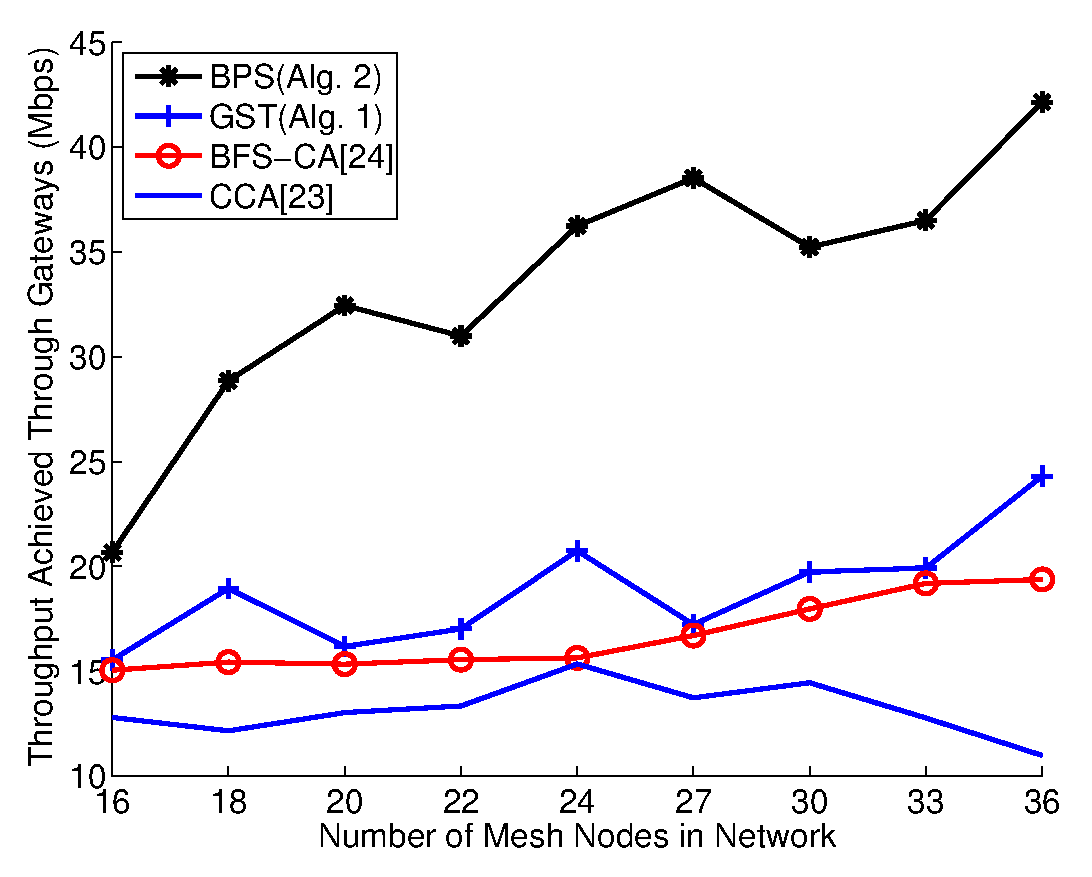
\includegraphics[width=2.3in]{figures/varysize}}
\hspace{-0.0in}
\subfigure[Varying Load, 30-Node Regular Grid]{
\label{fig:maxtpt}
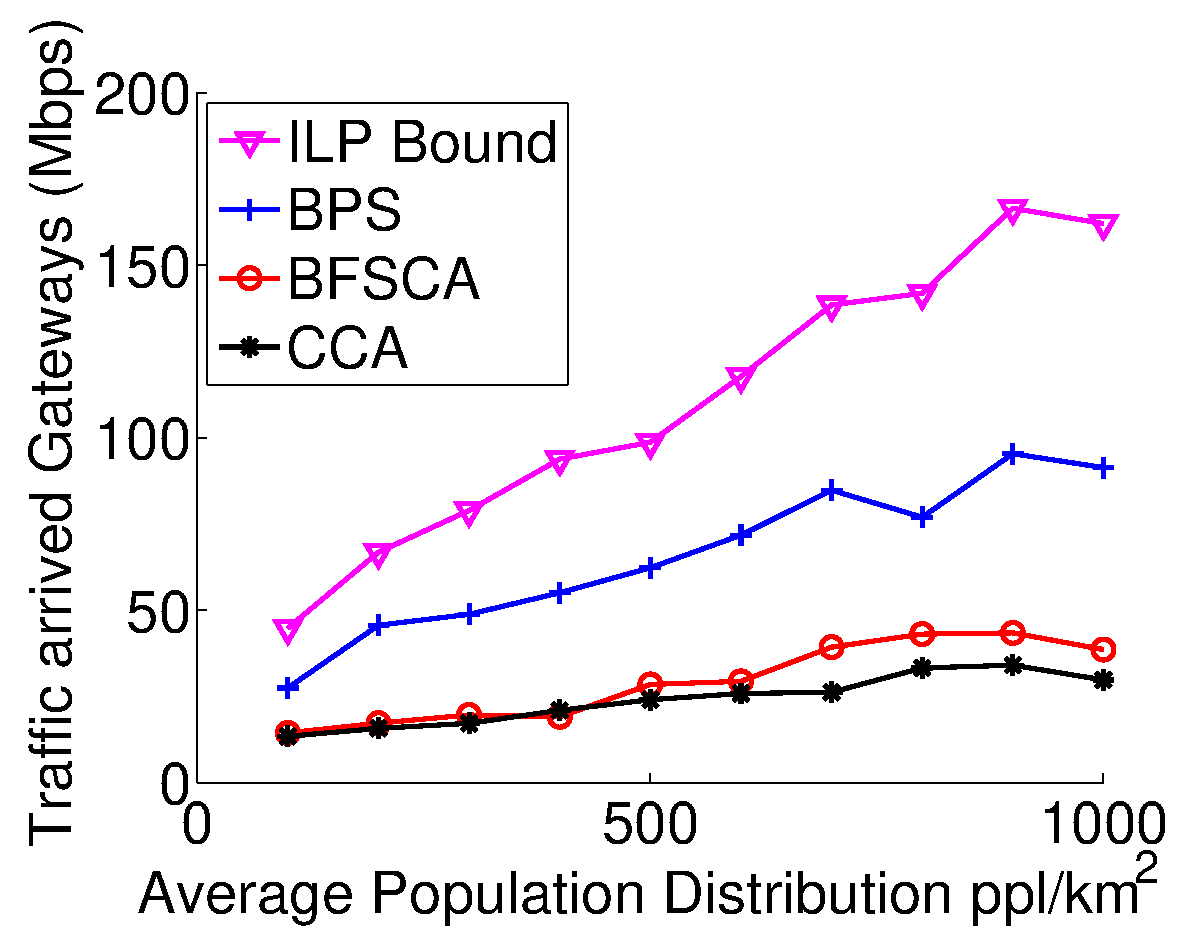
\includegraphics[width=2.3in]{figures/maxtpt.eps}}
\hspace{-0.0in}
\subfigure[BPS (Alg. 1), Varying WS Availability]{
\label{fig:wifiws}
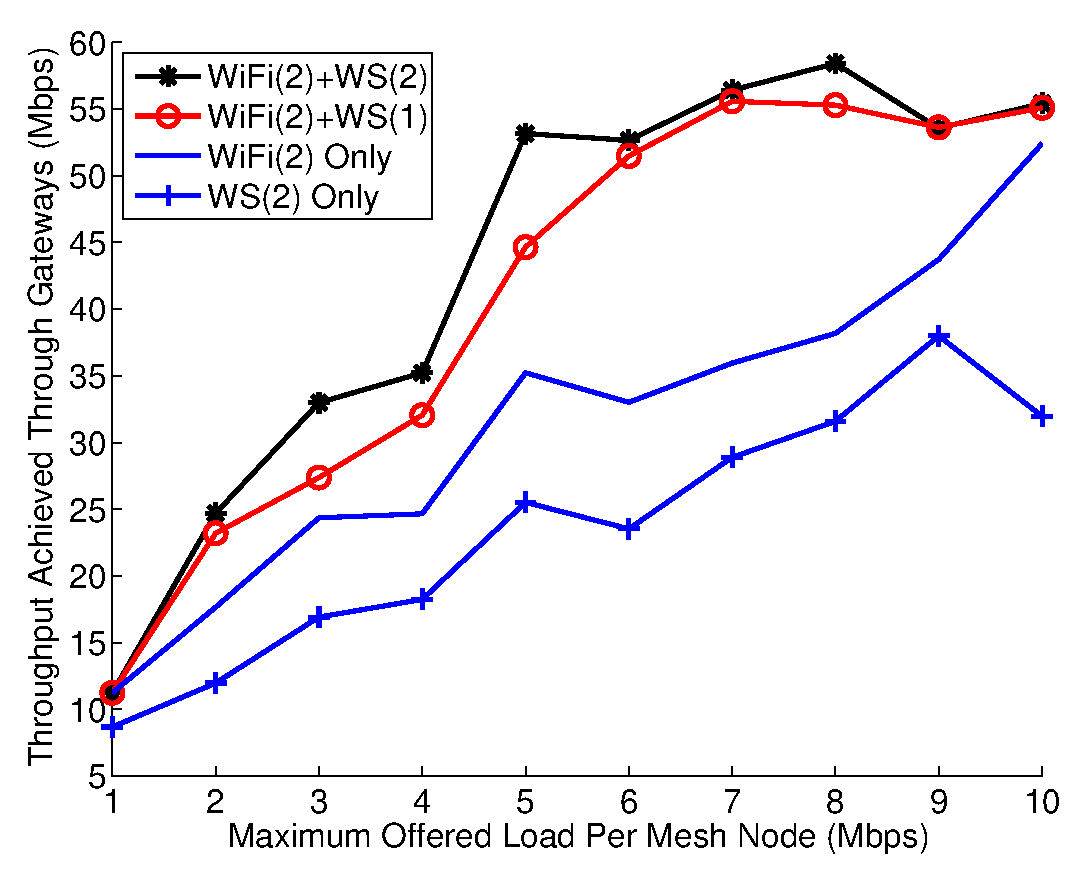
\includegraphics[width=2.3in]{figures/wifiws.eps}}
\vspace{-0.1in}
\caption{Performance in terms of gateway goodput for various offered loads, network sizes, and configurations of WiFi or white space (WS) channels.}
\label{fig:all3figs}
\vspace{-0.1in}
\end{figure*}

\begin{table*}
\centering % centering table 
\begin{tabular}{|l|c|c|c|c|c|c|c|c|c|c|c|} % creating 12 columns 
\hline %\hline % inserting double-line 
Bands/     & WiFi    & WS      & WS \& & WS \& &  WS \& & WS \& & WS \&      &  WS \&      & Multi-WS \& & Multi-WS \& & Multi-WS \& \\% [0.5ex]
Algorithms & Only    & Only    & WiFi  & WiFi  &  WiFi  & WiFi  & Multi-WiFi &  Multi-WiFi & WiFi        & WiFi        & Multi-WiFi  \\
\hline % inserts single-line 
% Entering 1st row 
WS (MHz)   &                                                        & 450,800 & 450 &  800  &  450   & 800               & 450    & 800      & 450,800     & 450,800     & 450,800     \\
\hline
WiFi (GHz) & 2.4, 5 &                                                             & 2.4 &  2.4  &  5   & 5               & 2.4, 5& 2.4, 5        & 2.4             & 5         & 2.4, 5     \\ % [0.5ex]
\hline
\hline % inserts single-line 
CCA~\cite{draves2004routing}                        & 3.1   &  7.3  & 8.2    &8.1    &8.3                &7.8     &   8.7    &   9.3&     9.0             &         11.9     &   14.4          \\      
\hline % inserts single-line                                                                                                       
BFS-CA~\cite{ramachandran2006interference}  & 8.9   &  6.2  & 7.9    & 9.0   & 13.6       & 13.8   &  14.9    &   13.8&      14.9           &      14.3       &       18.6      \\      
%\hline % inserts single-line                                                                                                      
%GST (Alg. 1)                                                            & 11.6  &   6.6 & 9.3    &   15.1&   15.8        &  14.4  &   16.6   &    14.1  &   18.8            &  15.0           &    25.1         \\      
\hline % inserts single-line                                                                                                     
BPS (Alg. 1)                                                            & 22.2  & 18.2  &  28.4  & 25.0  & 30.9          & 25.8   &   32.0  &  33.5       &     34.5            &      30.9       &       35.2      \\      
\hline % inserts single-line 
\end{tabular}    
\caption{Throughput achieved through Gateway nodes (Mbps) for various combinations of WiFi and Average Population Distribution = 600 $ppl/km^2$, Network Size = 30 mesh nodes).} % title name of the table 
% NEWClaim fix
\label{tab:2channelcombination}    
\vspace{-0.4in}
\end{table*}    

% ILP bound

Typically, clients and mesh nodes have diverse traffic patterns with
the download direction dominating the total traffic demand (e.g., consider
service agreements for cellular data or Internet connectivity). Hence, to
simplify the analysis and scale the ILP Bound to larger network sizes, we 
remove the uplink constraints while maintaining the downlink constraints.
We then randomly assign demand per mesh node with a maximum offered load
as specified in Fig.~\ref{fig:all3figs} and Table~\ref{tab:2channelcombination}.
We repeat the process 20 times, averaging the results of each of the
algorithms for the given network configuration.
%Most of the time clients of wireless network have different traffic demand. The uplink and dwon link traffic are equally occupy the channel capacity.
%Then we randomly assign demand of mesh nodes with a max offer load,
%calculate the scalable maximum throughput, then repeat the process 20 times.
%In the ILP bound, we keep the connectivity constraints in ~\ref{subsec:linearopt}. 
%To simiplify the process, we remove the uplink constraints and keep download demand constraints only. 
%The output is the average maximum throughput achieve gateways for the max offer load per mesh node.

In the first experiment, we consider different network sizes according to
the number of mesh nodes in the aforementioned regular grid. In particular,
we expect that as the network size grows, so too does the number of gateways,
producing a greater total gateway goodput. Fig.~\ref{fig:varysize} shows
the total gateway goodput when the 
% NEWClaim, ppl map to mesh
population distribution is 600 $ppl/km^2$
for the ILP formulation and the heuristic algorithms: 
{\it (i)} Common Channel Assignment (CCA) from~\cite{draves2004routing},
{\it (ii)} Breadth First Search Channel Assignment (BFS-CA) from~\cite{ramachandran2006interference},
%{\it (iii)} our first algorithm GST (Section~\ref{subsec:GST}), and
{\it (iv)} our algorithm BPS (Section~\ref{subsec:BPS}).
% NEWClaim fix, CCA, BFSCA
In CCA~\cite{draves2004routing}, two nodes will assign a channel for each other when there is a common
free channel for both of the nodes. In BFS-CA~\cite{tang2005interference}, a node will search all the 
available one-hop connections then choose the one has the largest capacity for a new assignment. 
These two methods assume the one-hop connections are equal when there is no assignment on the channel. 
In BPS, we both consider and leverage propagation differences of diverse bands.

%   \begin{figure}
%   %\vspace{-0.0in}
%   \centering
%   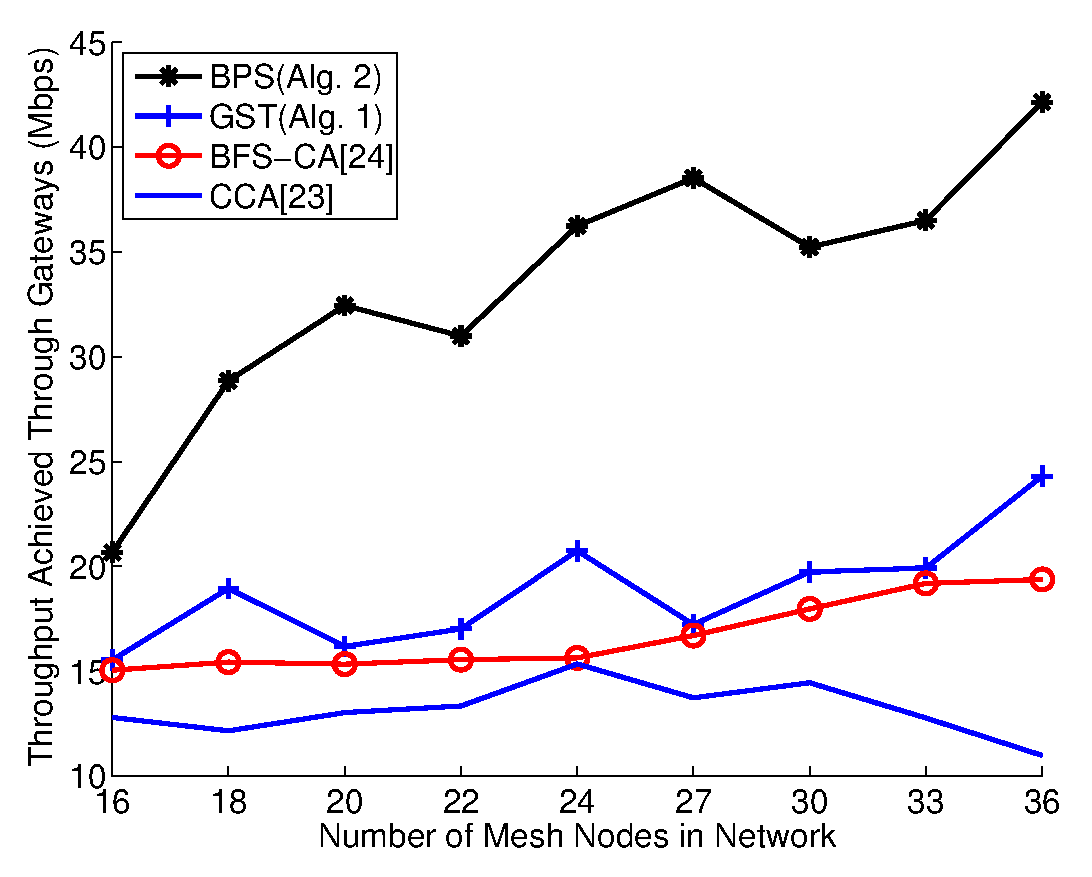
\includegraphics[width=74mm]{figures/varysize}
%   \vspace{-0.1in}
%   \caption{Uniform offered load per mesh node of 4 Mbps.}                                                                 
%   \label{fig:varysize}
%   %\vspace{-0.0in}
%   \end{figure}

In Fig.~\ref{fig:varysize}, we observe dips in the curves for all algorithms, 
representing the randomly generated demand.  The ILP Bound shows what could be
expected, that an increasing number of gateways produce an increase in total
gateway goodput.  However, we observe that the other algorithms are not able
to achieve such behavior for various reasons.  CCA increases the average
hop count the most, meaning that it was unable to find shorter routes to new
gateways.  
% NEWClaim,fix
%cond, while GST slightly outperforms BFS-CA, they both fail to 
%increase the reach of the gateway by attempting to optimize the first hop from
%the gateway. 
BFS-CA fails to increase the reach of the gateway by attempting to optimize the first
hop from the gateway.
Conversely, BPS alleviates the strain on these first-hop, bottleneck 
links, achieving up to 63\% of the ILP Bound. The key difference of BPS to the
ILP is that BPS only considers one path to a gateway node for each mesh node,
whereas the ILP allows multiple paths to the gateways.

Next, we consider a different form of scalability in our analysis.  Namely,
%we increase the maximum offered load per mesh node from 1 to 10 Mbps, whilea
% NEWClaim, fix
we increase the average population distribution from 150 to 1,500 per km$^2$, while
maintaining a 30-node regular grid topology. Fig.~\ref{fig:maxtpt} shows that
all of the algorithms are able to achieve comparable gateway goodput at 150
$ppl/km^2$.  However, as the population distribution increases, the ILP
and BPS diverge greatly from the remaining algorithms. Similar to 
Fig.~\ref{fig:varysize}, the wireless capacity around a gateway is quickly 
saturated if the algorithm is not focused on preserving that resource. Nonetheless,
we do observe a leveling off at approximately 60 Mbps offered load due to a
similar effect of the saturation of wireless capacity around the gateway node.
For BPS, this saturation point at 60 Mbps has a gateway goodput from 1.5 to 3.2 
times that of the remaining three algorithms, whereas the ILP Bound has between
2.7 and 4.18 times the gateway goodput. BPS has a performance of 75\% of the ILP
Bound, on average.

%   \centering
%   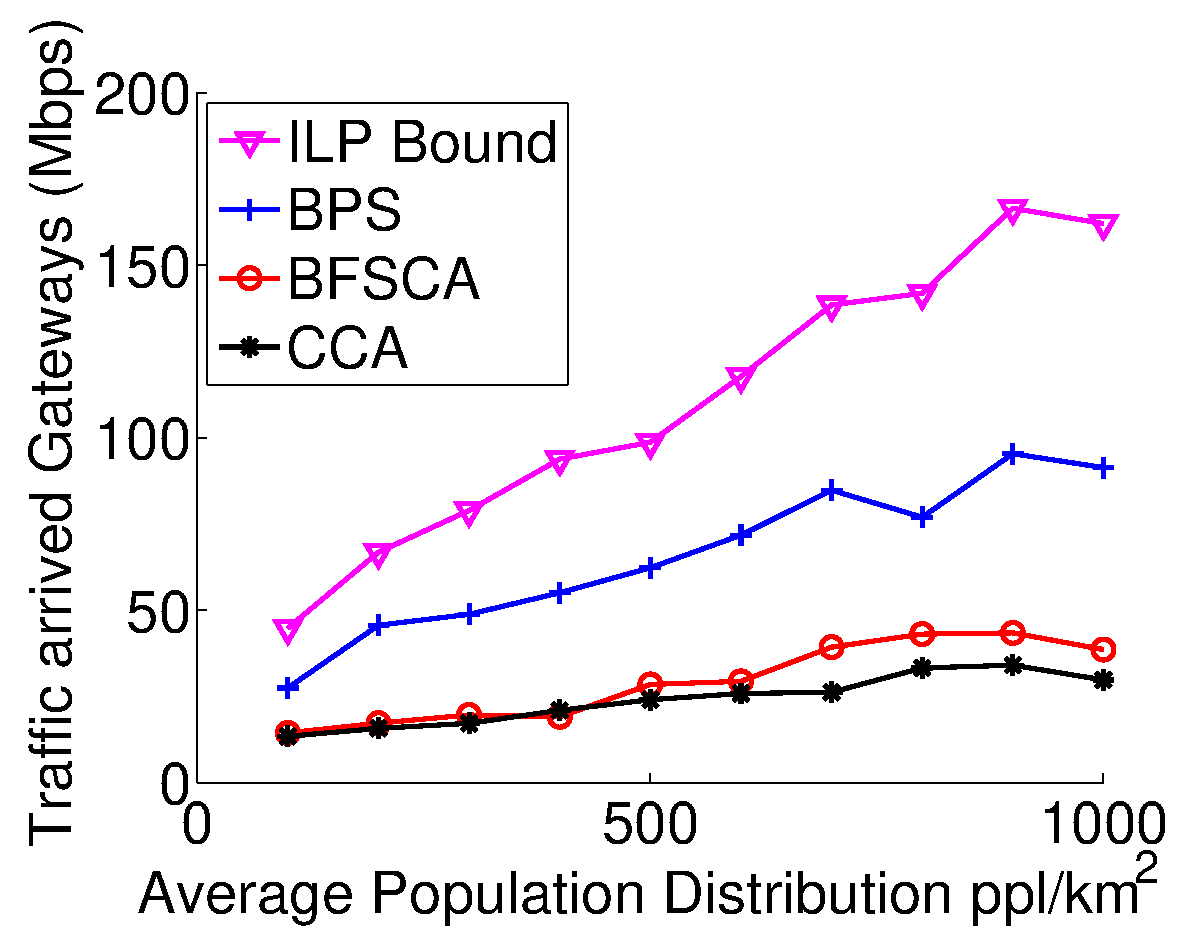
\includegraphics[width=74mm]{figures/maxtpt}
%   \vspace{-0.1in}
%   \caption{Varying maximum offered load for a 30-node regular-grid mesh topology.}                                                                               
%   \label{fig:maxtpt}
%   %\vspace{-0.0in}
%   \end{figure}
 
%   BPS performs better than the other 3 algorithms since during the channel assignment process, it is already optimize the paths from further nodes to gateways make it possible to ship data from these nodes. But as the max offer load increase, all the channel assignment suffer the bottle neck of link capacity.
%   GST is trying to optimizing the output of BFS-CA, reducing the hop counts and interference of each hop layer. However, since the 1 hop layer has been assigned throughput BFS-CA which is the bottle neck for the capacity of the network.

WhiteMesh networks will be deployed across a vast array of environments, from
rural to urban areas.  Each of these areas will have varying amounts of user 
demand in proportion to the population densities.  However, since a greater
number of TV stations exist in urban areas, the available white space bands are
often inversely related to the population density. To capture these varying
degrees of demand and white space availability we consider three likely scenarios
and one final scenario for comparison purposes: {\it (i)} two WiFi bands (2.4 and
5.8 GHz) with two white space channels (450 and 800 MHz), {\it (ii)} two WiFi
bands (2.4 and 5.8 GHz) with one white space channel (450 MHz), {\it (iii)} two
WiFi bands (2.4 and 5.8 GHz) without any white space channels, and {\it (iv)}
two white space bands (450 and 800 MHz) with no WiFi bands (for comparison).

In Fig.~\ref{fig:wifiws}, we consider the performance of BPS in the four aforementioned
scenarios of varying white space availability with varying offered load from 1 to 10 Mbps,
representing different population densities. A regular, 30-node grid is again used.
Immediately, we observe that the WiFi-only scenario has greater gateway goodput
than the white-space-only scenario.  This is due to the lack of spatial reuse achieved
by white spaces.  Interestingly, however, the joint use of both white space and WiFi
bands has significant gains over the single type of band scenarios (37\% greater than
WiFi and 85\% over white space, on average).  This can be explained in part
because the joint use of WiFi and white space has more total bands to use.  However,
we will see in Table~\ref{tab:2channelcombination} that even with the same number of
available bands (2), the combination of the two can achieve significant gains over
scenarios with only WiFi or white space.   

Table~\ref{tab:2channelcombination} describes the achieved gateway goodput for various
combinations of WiFi and white space bands with a maximum offered load of 4 Mbps and
a regular 30-node grid. The second reason for the gains in Fig.~\ref{fig:wifiws} 
with WiFi and white space is completely isolated in this scenario. Consider the case where we use a white space band of 450 MHz 
and a WiFi band of 5.8 GHz.  
% NEWClaim, fix
%Note that, even
%with the same bandwidth, transmission power, and antenna gain, the joint use of 
%these bands allows 15.8 Mbps of gateway goodput with GST versus 11.6 Mbps for
%WiFi only and 6.6 Mbps for white space only topologies with gains of 36\% and 140\%,
%respectively. 
With BPS and the same bandwidth, transmission power, and antenna gain, we achieve 
30.9 Mbps of gateway goodput through jointly use of these bands, 
versus 22.2 Mbps with WiFi only or 18.2 Mbps for white space only with gains of 
40\% and 70\%, respectively. If we have one channel in a white space band and one 
channel in a WiFi band, then we could use the advantage of WiFi for spatial reuse
and white spaces to reduce the hop count. These two points become more critical at
different points in the WhiteMesh topology. For the sake of completeness, we present
many other scenarios which could be interesting for WhiteMesh deployments.


%Our results also shows the importance of channel selection of multiband. ~\ref{tab:2channelcombination} shows when 2 radios could be used, the better combination would be a higher frequency and a lower frequency which could combine the advantage of reduce interference in the network through high frequency link and benefit from decrease hop count through low frequency link. 
%Two low frequency channel, as in ~\ref{tab:2channelcombination}, will bring more interference to the network.
%In this scenario, the performance is even worse than use WiFi channel only. 
%The reason two low frequency channels has better performance than WiFi only in CCA due to the channel assignment fails to connect all mesh node to the gateways make there exist some offer load can not be shipped to gateways.
%So a smart way to choose channels is to select a set of channels in different band rather than select channels has the same propagation characteristics.

   % Use table to replace the hint graph


				   %				   \begin{table}[h] 
				   %				   \centering % centering table 
				   %				   \begin{tabular}{|p{1.2cm}| p{1.2cm} | p{0.9cm} | p{1.2cm} |p{1.1cm}|p{1.2cm}|} % creating 10 columns 
				   %				   \hline %\hline % inserting double-line 
				   %				   \multirow{2}{*}{Type} & \multirow{2}{*}{Bands} & \multicolumn{4}{c|}{Algorithms}   \\% [0.5ex]
				   %				   \cline{3-6}
				   %				   %  \hline
				   %				   & & CCA[23] & BFSCA[24] & GST(Alg.1) & BPS(Alg.1) \\ [2ex]
				   %				   % \\ [0.5ex] 
				   %				   \hline % inserts single-line 
				   %				   WiFi Only & $2.4+5G$ & 3.0912 & 8.9460 & 11.5934 & 22.2179 \\ [2ex]
				   %				   \hline % inserts single-line 
				   %				   WS Only & $450+900M$ & 7.3428 & 6.2115 & 6.5567 & 18.1946 \\[2ex]
				   %				   \hline % inserts single-line 
				   %				   \multirow{4}{*}{\begin{minipage}{0.5in}WiFi +WS\end{minipage}} & 2.4G+450M & 8.2168 & 7.9206 & 9.2521 & 28.4069 \\[2ex]
				   %				   \cline{2-6} % inserts single-line 
				   %				   & $2.4G+900M$ & 8.1321 & 8.978 & 15.0802 & 24.985 \\[2ex]
				   %				   \cline{2-6} % inserts single-line 
				   %				   & $5G+450M$ & 8.3416 & 13.5729 & 15.8455 & 30.9351 \\[2ex]
				   %				   \cline{2-6} % inserts single-line 
				   %				   &$ 5G+900M$ & 7.8412 & 13.8290  & 14.4036 & 25.8345 \\[2ex]
				   %				   \hline % inserts single-line 
				   %				   WiFi+ Multi-WS &$2.4G+450M+900M$  & 8.9788 & 14.9167 & 18.7859& 34.5374 \\[2ex]				   %				   \hline % inserts single-line 
				   %				   Multi-WiFi+WS & $2.4G+5G+450M$ & 8.6892 &14.9167 &16.6344 &31.9532  \\[2ex]
				   %				   \hline % inserts single-line 
				   %				   Multi-WiFi+Multi-WS & $2.4G+5G+450M+900M$ &14.3703  & 18.6406 &25.0988 & 53.1671 \\[2ex]
				   %				   \hline % inserts single-line 
				   %				   \end{tabular} 
				   %				   \label{tab:2channelcombination} 
				   %				   \caption{Various combinations of WiFi and White Space mesh topologies (offered load = 5Mbps, network size = 30).} % title name of the table 
				   %				   \vspace{-0.1in}
				   %				   \end{table} 
				   %
				   %
				   %\begin{table*}
				   %				   \centering % centering table 
				   %				   \begin{tabular}{|p{1.3cm}| p{1.3cm} | p{1.3cm} | p{1.3cm} |p{1.3cm}|p{1.3cm}|} % creating 10 columns 
				   %				   \hline %\hline % inserting double-line 
				   %				   \multirow{2}{*}{Type} & \multirow{2}{*}{Bands} & \multicolumn{4}{c}{Algorithms}   \\% [0.5ex]
				   %				   \cline{3-6}
				   %				   %  \hline
				   %				   & & CCA[23] & BFSCA[24] & GST(Alg.1) & BPS(Alg.2) \\ [2ex]
				   %				   % \\ [0.5ex] 
				   %\end{table}
				   %


%The number of radio equipped on a node in mesh network also abstract ISP attention. 
%The result shows in ~\ref{fig:varyradios}, BPS has the best performance over other algorithms. 
%Increasing radios do improve the performance of network. 
%As more radios equipped in the network, the benefit would be decrease in most scenario. 
%There is a trade off between performance of more radios and cost increasing.
%In one radio scenario, BPS outperforms CCA, but fails in completion of BFS-CA and GST.
%But in multi-radio scenarios, BPS always outperforms the other methods.


%\begin{figure}
%%\vspace{-0.0in}
%\centering
%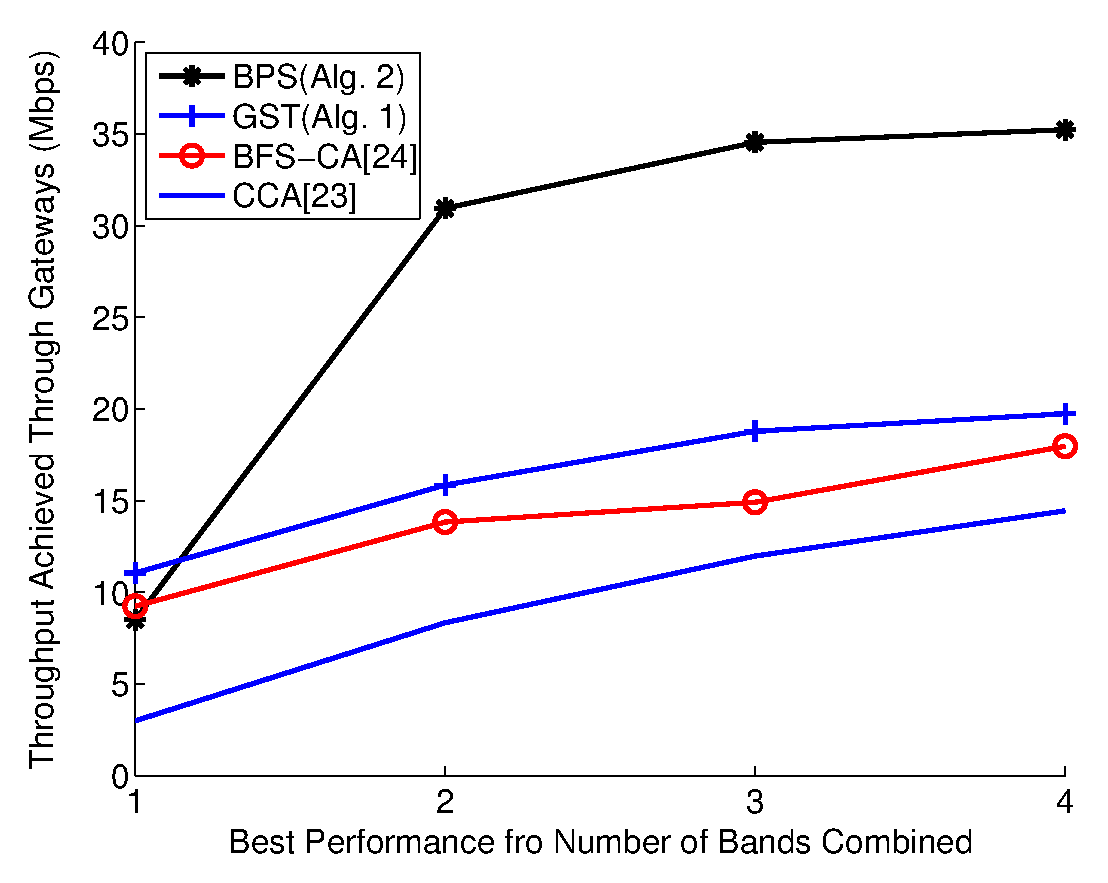
\includegraphics[width=74mm]{figures/varyradios}
%\vspace{-0.1in}
%\caption{Varying radios in 30-node regular-grid of 4 Mbps.}                                                                               
%\label{fig:varyradios}
%%\vspace{-0.0in}
%\end{figure}





%In ~\ref{fig:wifiws}, the performance of 4 different type of band combination is shown. 
%The four curves are WiFi Only (2.4,5 GHz), WS Only (450,800 MHz), WS (450 MHz) + Multi-WiFi(2.4 GHz), Multi-WS(450, 800 MHz) + Multi-WiFi(2.4, 5 GHz). 
%Increasing radios do help to improve the performance, but with the same radios and bandwidth, WiFi and white space combination could outperform only WiFi and only white space performance.

%\begin{figure}
%%\vspace{-0.0in}
%\centering
%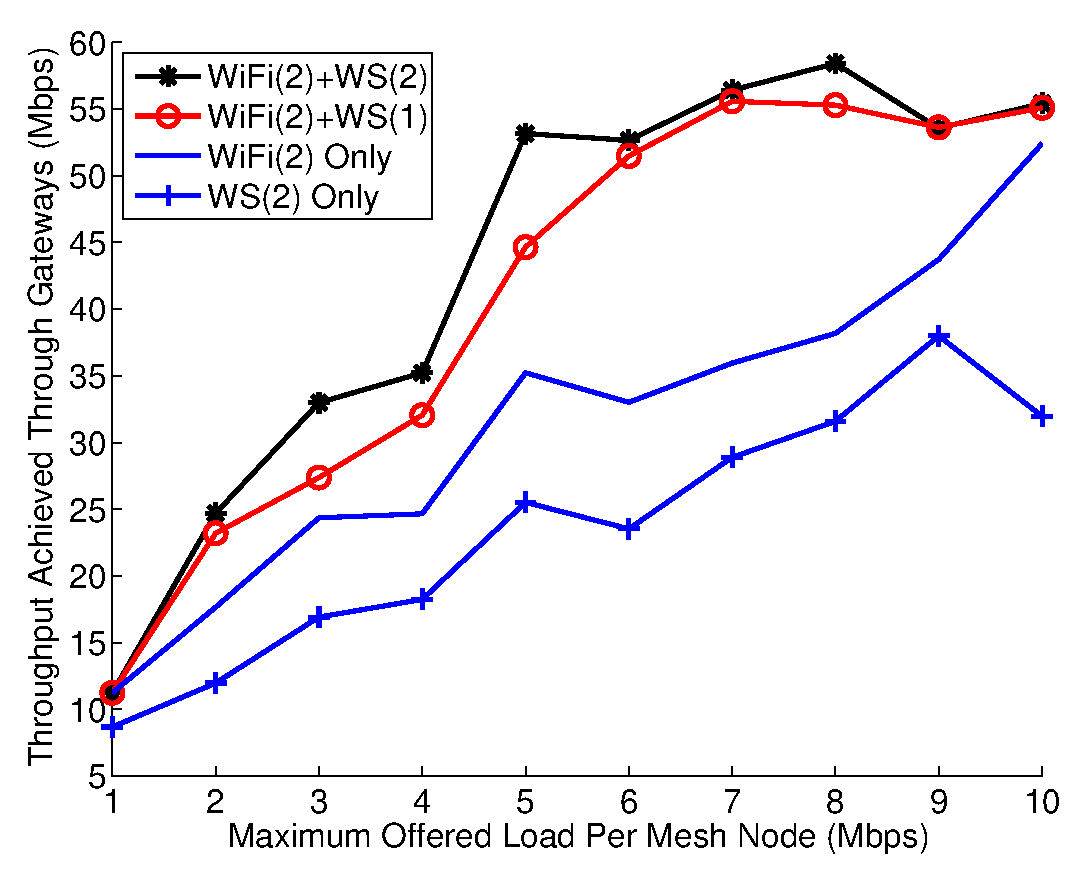
\includegraphics[width=74mm]{figures/wifiws}
%\vspace{-0.1in}
%\caption{BPS (Alg. 2) performance with two total channels of WiFi or white space (WS) with varying offered load from x mesh nodes.}
%\label{fig:wifiws}
%%\vspace{-0.0in}
%\end{figure}
